\section{Objectif}
\label{chap:Objectif}

L'objectif de ces Travaux Pratique est de démontrer les capacités du PSoC est de se familiariser avec le
 PSOC creator en tant que plateforme de développement embarquée,développer les compétences en programmation du PSOC
identifier et résoudre des problèmes de fonctionnement du PSOC et creer des circuit electronique
\\

\section{Activité n°1:Blinking led}
\label{chap:Activité n°1:Blinking led}
Dans cette partie on va découvrir le logiciel PSoC Creator 3.0
\subsection{Etude Theorique}
\label{sec:Etude Theorique}
\begin{itemize}
    \item \textcolor{red}{\textbf{Configuration matérielle:}} Le PSOC est une plateforme de développement embarquée flexible, offrant différents types de broches d'entrée/sortie (E/S).
     Pour faire clignoter une LED, vous devez connecter la LED à une broche de sortie du PSOC 
    \item \textcolor{red}{\textbf{Programmation:}} Le PSOC est programmé à l'aideue langage C dans l'environnement de développement spécifique  PSoC Creator.
      l'état de la broche de la led  configurée en sortie en changer en  lui attribuant une valeur logique de haut (HIGH) ou de bas (LOW) Grace au PWM
\end{itemize}


\subsection{Manipulation}
\label{sec:Manipulation}

\begin{itemize}
    \item \textbf{Lancer le logiciel Psoc Creator}
      \begin{figure}[htp]
        \centering
        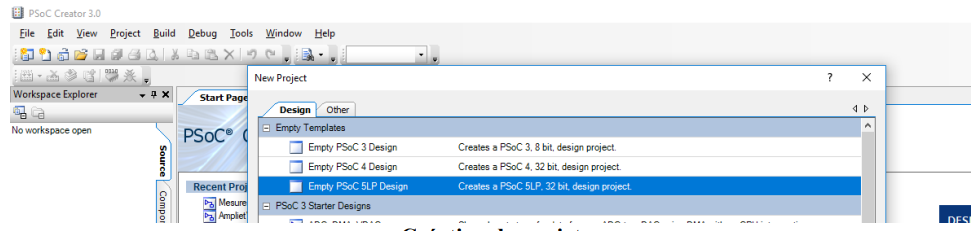
\includegraphics[width=1.1\textwidth]{images/lancement.png }
        \caption{Lancement logiciel }
        \label{fig:example1}
      \end{figure}

    \item \textbf{Crée un nouveau projet et un nouveau fichier} 
    \item \textbf{Configuration matérielle:}
    \item \textbf{Dessiner la structure de notre application dans le fichier TopDesign}
    \begin{figure}[htp]
        \centering
        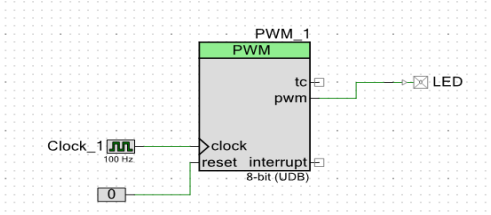
\includegraphics[width=1.1\textwidth]{images/schema1.png }
        \caption{Schema pour une Led }
        \label{fig:example2}
      \end{figure}
    \\
    \item \textbf{Affectation des broches du circuit dans le fichier .cydwr}
    \\
    \begin{figure}[htp]
        \centering
        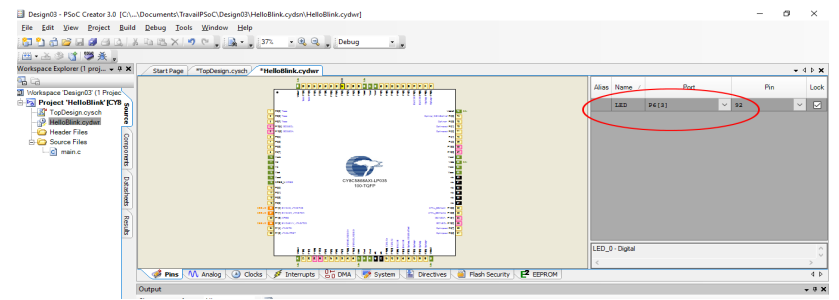
\includegraphics[width=1.1\textwidth]{images/broche.png }
        \caption{Selection des broches }
        \label{fig:example3}
    \end{figure}
    \item \textbf{Ajouter la commande  PWM Start() au fichier main.c}
    \item \textbf{Choisir les valeurs adequates du signal PWM dans les parametres en fonction de la durée souhaitée}
    \item \textbf{Compiler les fichiers }
    \item \textbf{Relier la carte d’évaluation au PC à l’aide de la prise USB et cliquer sur programm}
\\
\begin{figure}[htp]
    \centering
    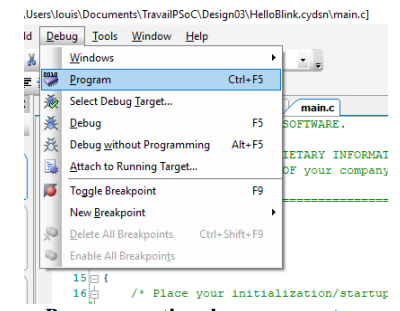
\includegraphics[width=10cm]{images/click.png }
    \caption{Lancer le Televersement }
    \label{fig:example4}
  \end{figure}
\end{itemize}
\subsection{Résultat obtenue}
\label{sec:Résultat obtenue}

\begin{figure}[htp]
    \centering
    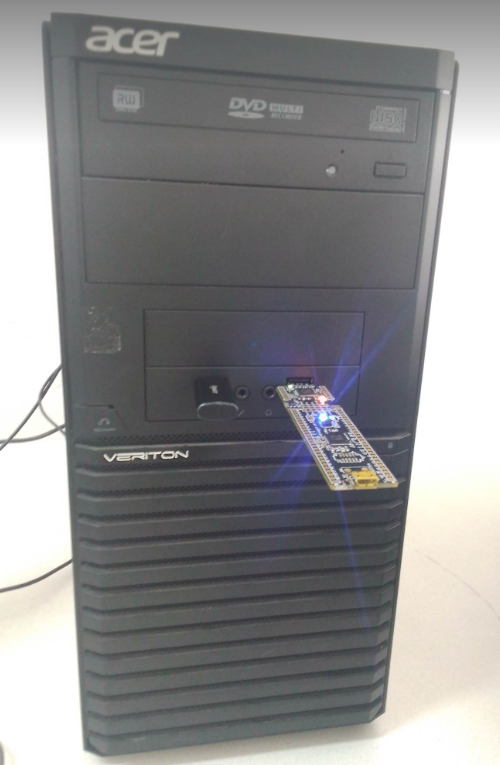
\includegraphics[width=5cm]{images/led.png }
    \caption{ Resultat:Led bleue clignote }
    \label{fig:example5}
  \end{figure}

La diode de la carte clignote chaque seconde grâce à la commande PWM-1-Start et  PWM-1-Sleep pour l’arrêt.
 
\subsection{Interpretation}
\label{sec:Interpretation}
\todo[inline]{En connectant correctement la LED à la broche de sortie appropriée, le projet permet de confirmer 
que la communication entre le PSOC et la LED fonctionne correctement.
clignotement de LED peut être utilisé pour tester le bon fonctionnement du PSOC et des composants périphériques. 
Il permet de s'assurer que le système est capable de générer des signaux de sortie et de contrôler des dispositifs externes tels que des LED.
}

\section{Activité n°2 :Clignotement de deux leds en alternance}
\label{chap:Activité n°2 :Clignotement de deux leds en alternance}
Dans cette partie on va faire clignoter deux diodes de couleurs différentes (une rouge et une verte) de manière alternative afin 
de créer un effet de clignotement 

\subsection{Etude Theorique}
\label{sec:Etude Theorique}
\begin{itemize}
    \item \textcolor{red}{\textbf{Configuration matérielle:}} Choisissez deux broches GPIO disponibles sur le PSoC pour connecter les LED.
     Assurez-vous de noter les numéros de broche pour référence ultérieure.Trouver l'anode et la cathode de chaque LED
    \item \textcolor{red}{\textbf{Programmation:}}l'environnement de développement intégré (IDE) du PSoC
     comme PSoC Creator,choisir la bonne carte et créez un nouveau projet.
\end{itemize}


\subsection{Manipulation}
\label{sec:Manipulation}
\begin{itemize}
    \item \textbf{Lancer le logiciel Psoc Creator:}
    Lancez PSoC Designer et créez un nouveau projet en sélectionnant 
    le microcontrôleur PSoC adapté à votre modèle spécifique.
    \item \textbf{Ajoutez les composants nécessaires: } 
    Dans l'onglet "Component Catalog"
    recherchez et ajoutez les composants requis pour les deux diodes
    \begin{figure}[htp]
        \centering
        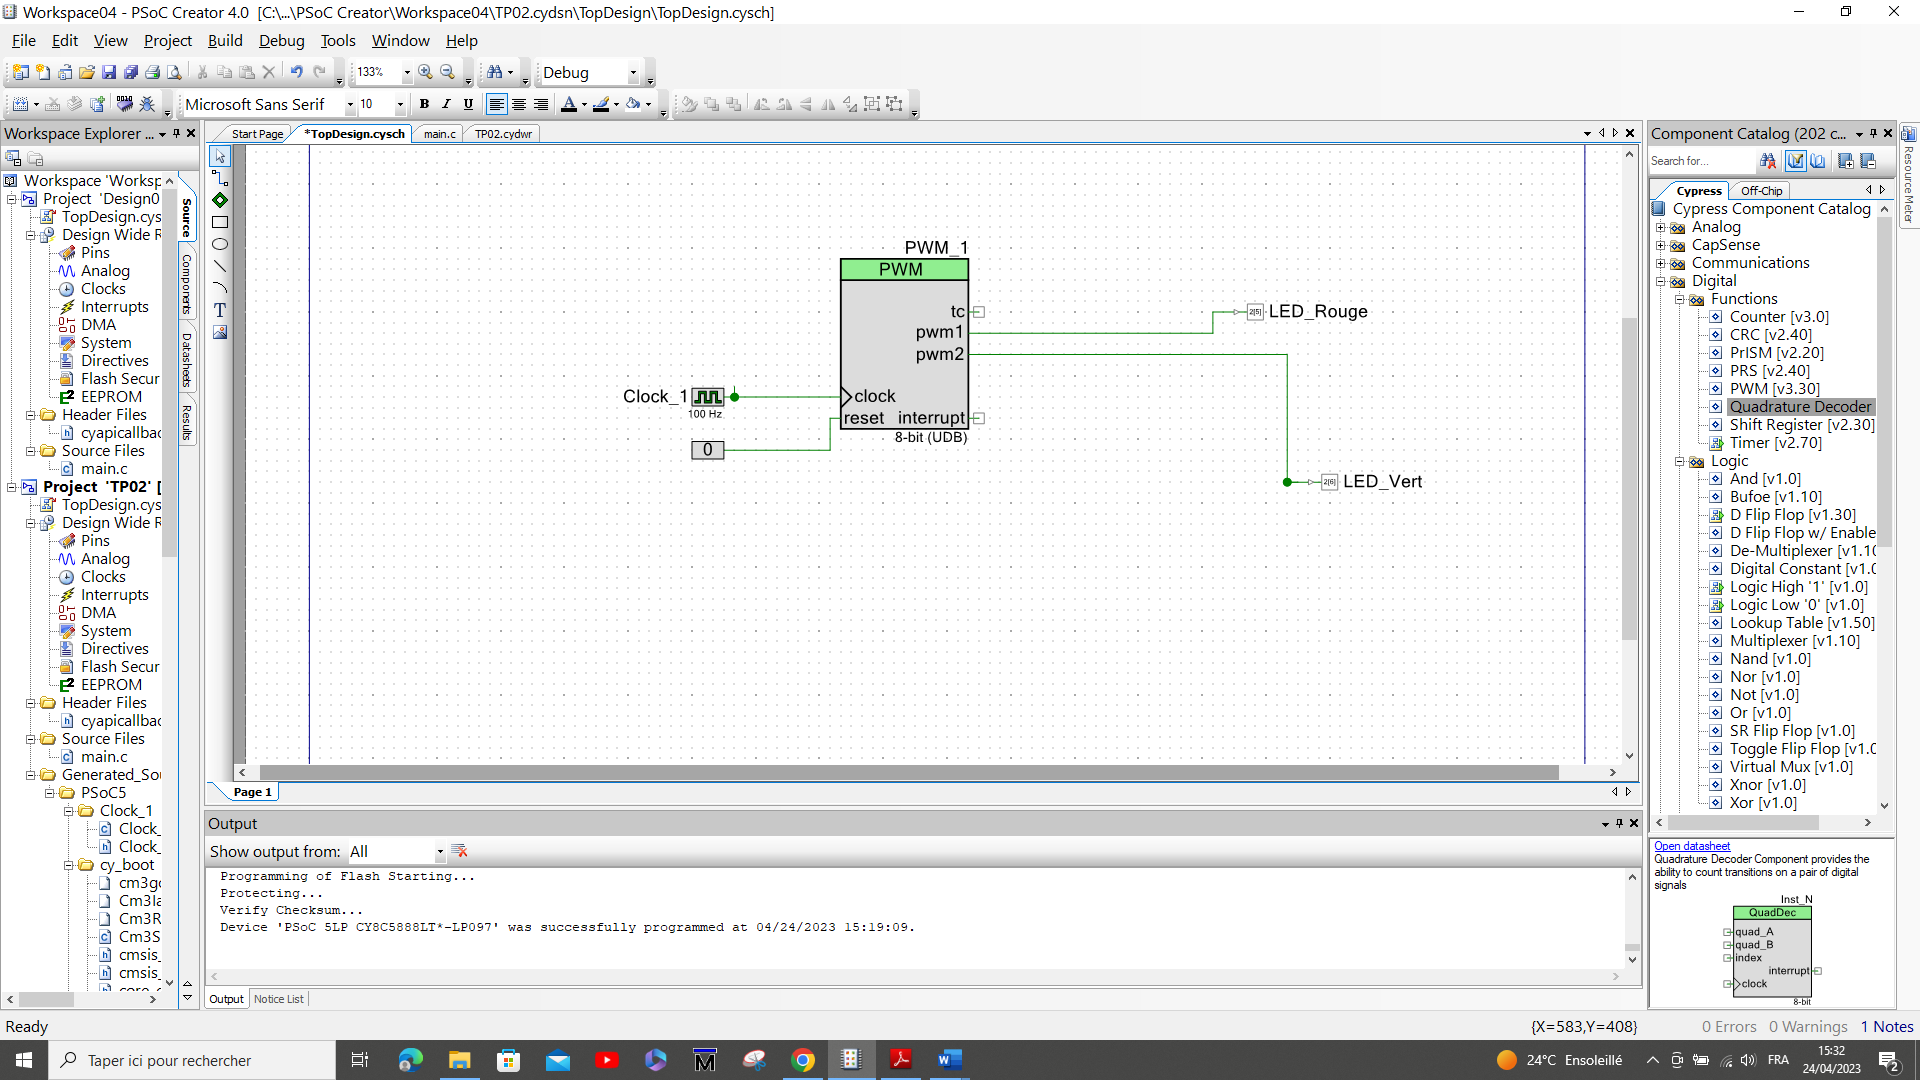
\includegraphics[width=10cm]{images/two.png }
        \caption{Schema pour 2 Leds }
        \label{fig:example6}
      \end{figure}
    \item \textbf{Configuration des broches de sortie dans .cydwr}
    veillé à ce que les broches soient définies en mode numérique et en tant que sorties.
    \begin{figure}[htp]
        \centering
        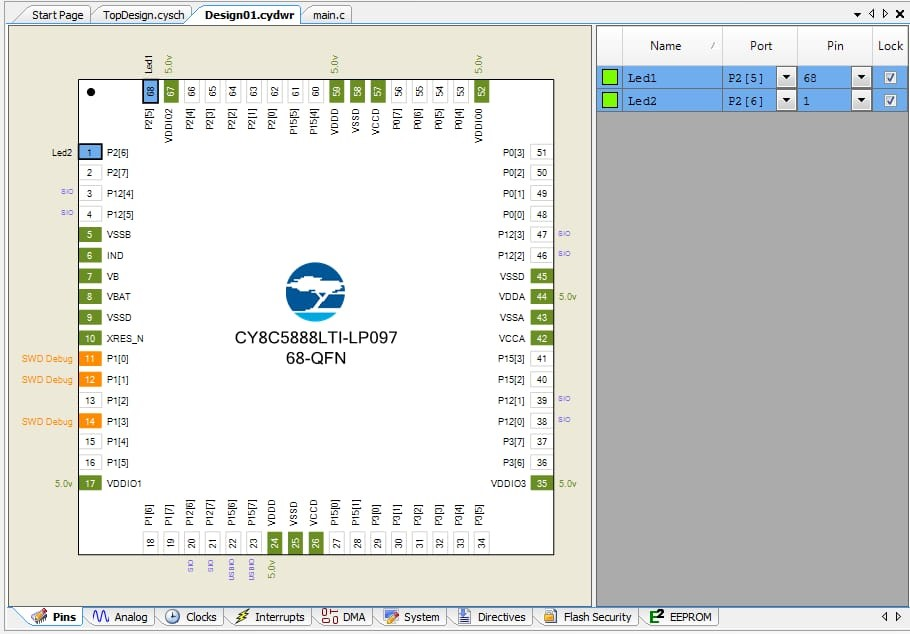
\includegraphics[width=10cm]{images/broche2.jpg }
        \caption{Affectation des broches }
        \label{fig:example7}
      \end{figure}
    \item \textbf{Ecrire le code du projet fichier main.c}
    \begin{figure}[htp]
        \centering
        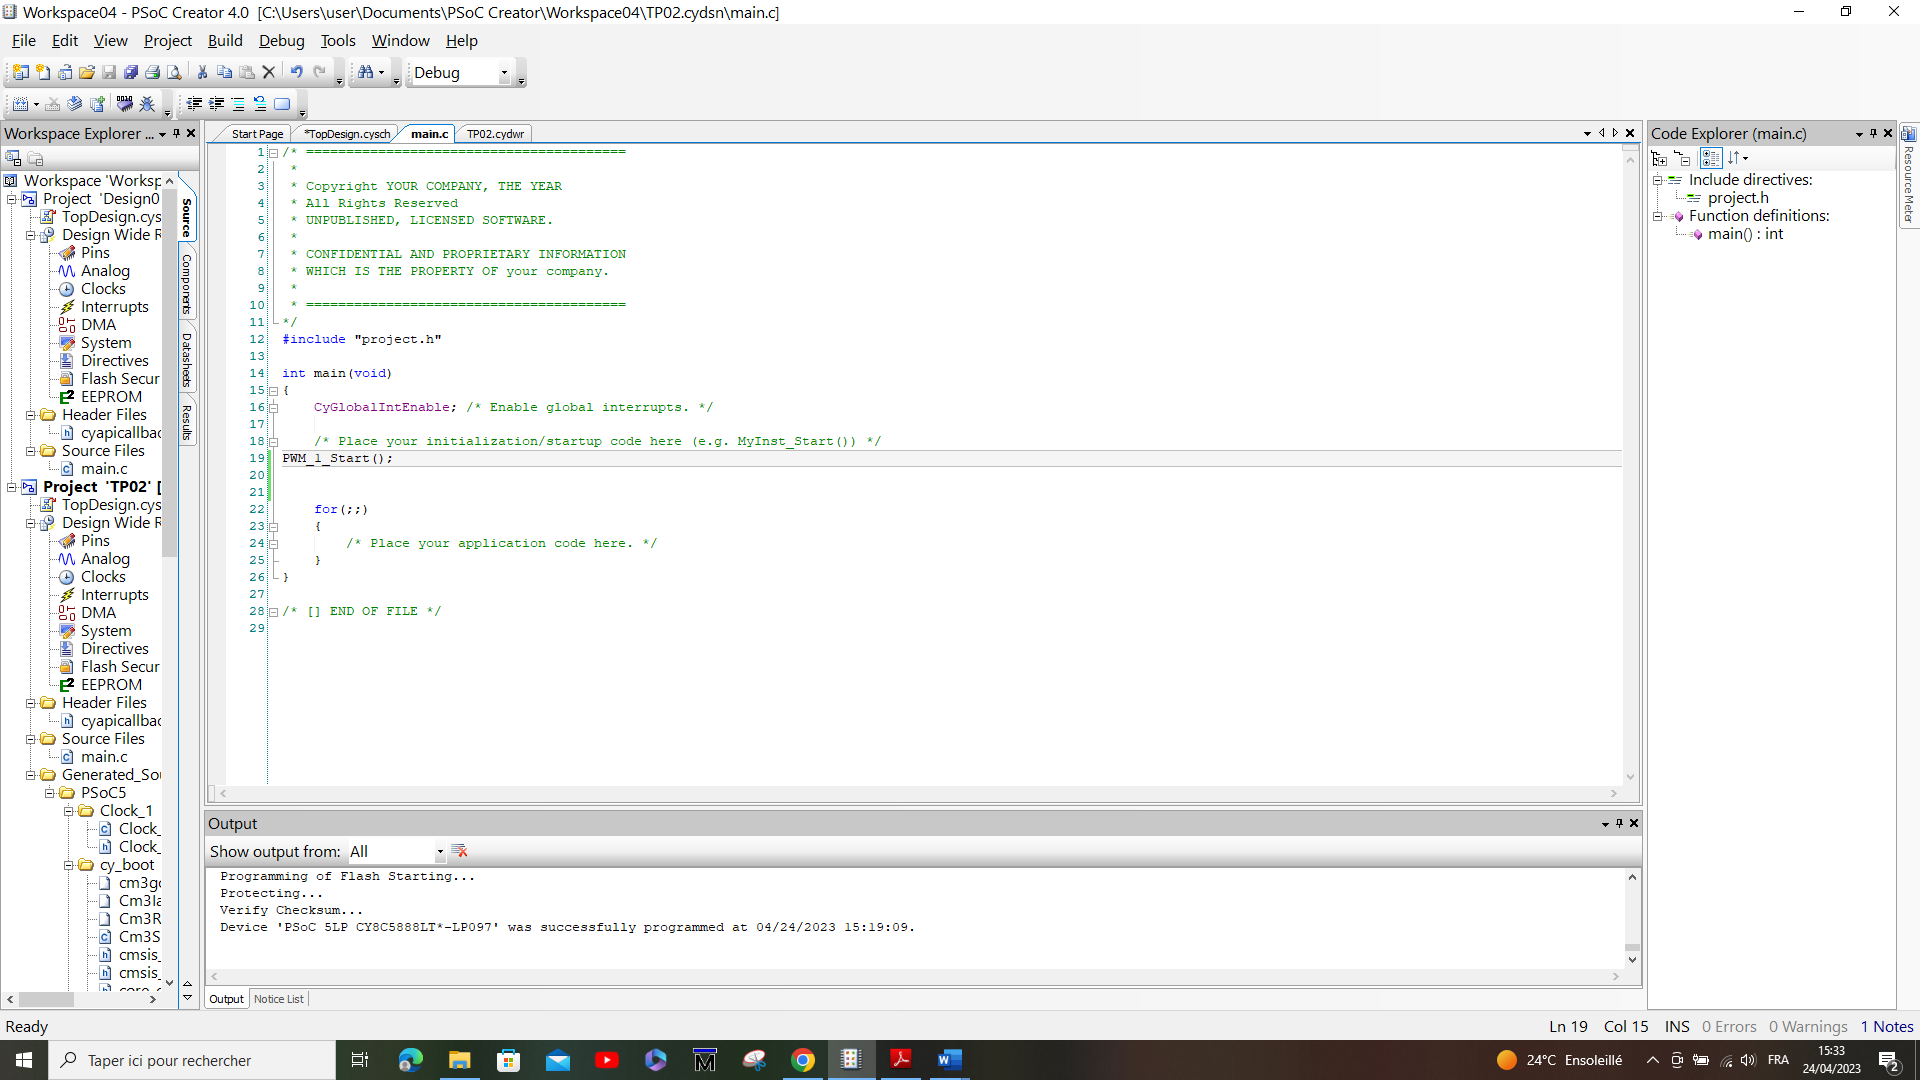
\includegraphics[width=15cm]{images/codetwo.png }
        \caption{Code main.c }
        \label{fig:example8}
      \end{figure}
    \item \textbf{Effectuer le montage et Televersement }
    \item \textbf{Choisir les valeurs adequates du signal PWM dans les parametres tout en alternant les periodes HIGH} 
\end{itemize}
\subsection{Résultat obtenue}
\label{sec:Résultat obtenue}
Après avoir programmé le PSoC, les deux diodes devraient 
clignoter de manière alternative toutes les 500 millisecondes.
\begin{figure}[htp]
    \centering
    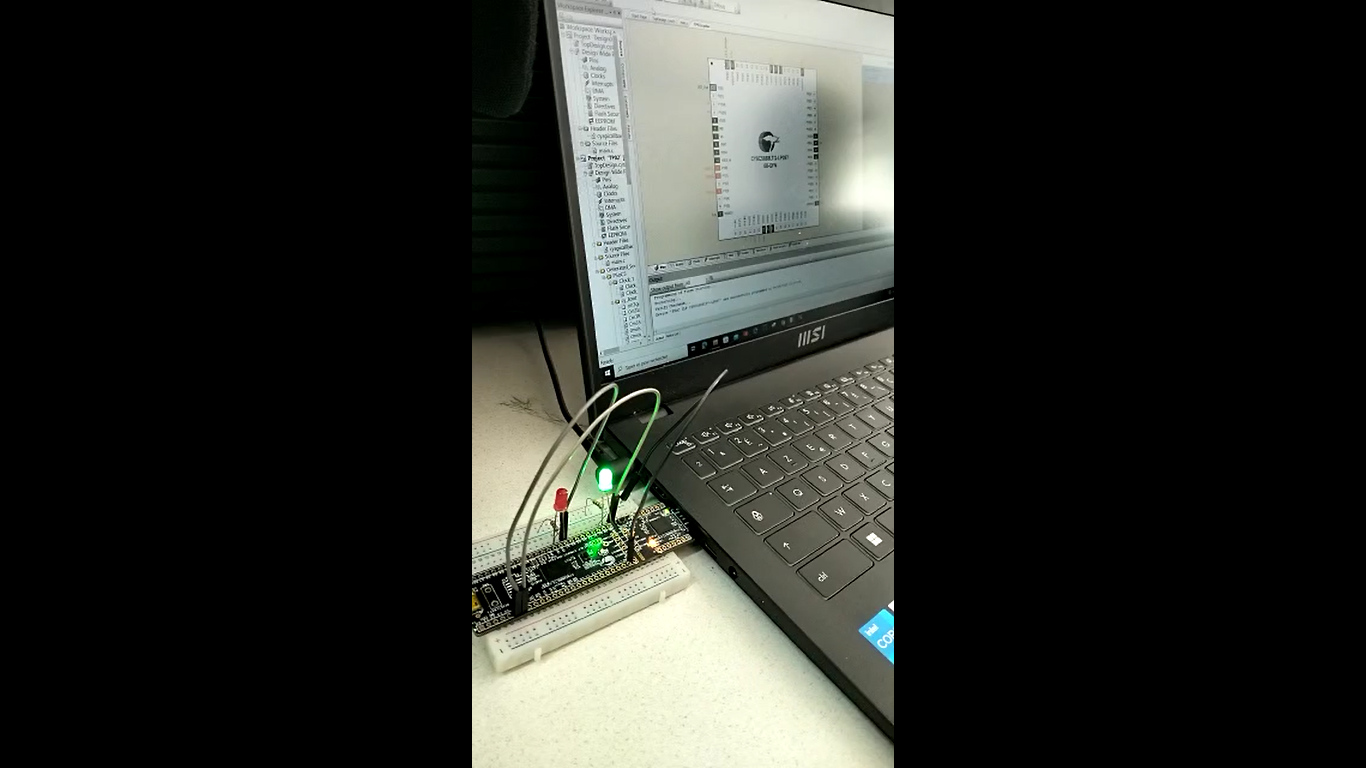
\includegraphics[width=15cm]{images/alternance.png }
    \caption{ Resultat:Clignotement en alternance}
    \label{fig:example9}
  \end{figure}

Les diodes clignote chaque seconde grâce à la commande PWM-Start et  PWM-Sleep pour l’arrêt.
 
\subsection{Interpretation}
\label{sec:Interpretation}
\todo[inline]{Le PSoC peut etre utilisé pour générer des signaux de sortie pour piloter les LED et
 démontre la flexibilité du PSoC dans la gestion des entrées/sorties.L'objectif principal est 
 de fournir une indication visuelle ou une interaction avec l'utilisateu
}
 \section{Activité n°3 : Compteur à sept segments }
 \label{chap:Activité n°3 :Compteur à sept segments }
 Dans ce projet, le PSoC sera utilisé pour contrôler l'afficheur à sept 
 segments et afficher des chiffres ou des caractères spécifiques. 
 Le PSoC offre une grande flexibilité et des fonctionnalités intégrées, ce qui 
 facilite la génération de signaux de commande appropriés pour l'afficheur.
 
 \subsection{Etude Theorique}
 \label{sec:Etude Theorique}
 \begin{itemize}
     \item \textcolor{red}{\textbf{Configuration matérielle:}} Choisissez un afficheur à sept segments compatible, 
     qui peut être de type anode commune ou cathode commune.Noter les connexions spécifiques pour chaque segment A, B, C, D, E, F, G
     et le point décimal DP de l'afficheur.
     \item \textcolor{red}{\textbf{Configuration matérielle:}}l'environnement de développement intégré (IDE) du PSoC
      comme PSoC Creator,choisir la bonne carte et créez un nouveau projet.
 \end{itemize}
 
 
 \subsection{Manipulation}
 \label{sec:Manipulation}
 \begin{itemize}
     \item \textbf{Lancer le logiciel Psoc Creator:}
     Lancez PSoC Designer et créez un nouveau projet en sélectionnant 
     le microcontrôleur PSoC adapté à votre modèle spécifique.
     \item \textbf{Ajoutez les composants nécessaires: } 
     Dans l'onglet "Component Catalog"
     recherchez et ajoutez les composants requis pour les deux diodes
     \begin{figure}[htp]
         \centering
         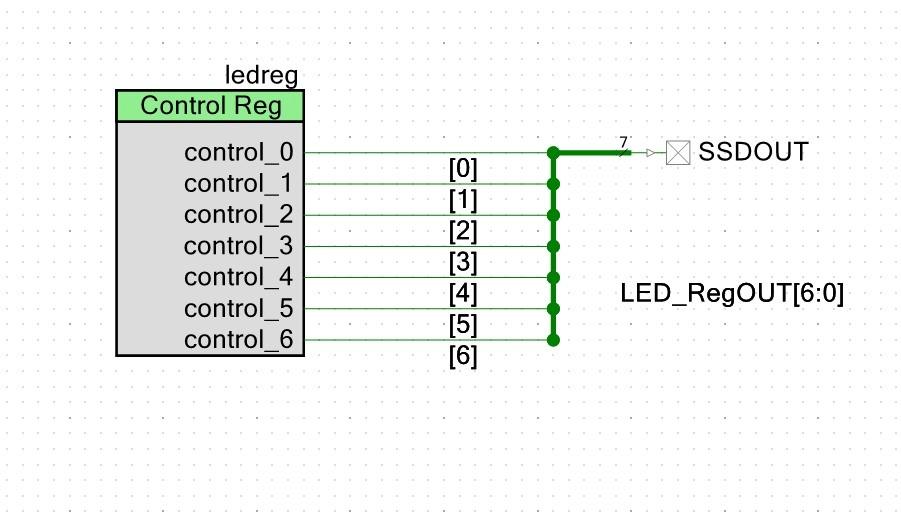
\includegraphics[width=10cm]{images/schema3.jpg }
         \caption{Schema pour Afficheur 7 Segments }
         \label{fig:example10}
       \end{figure}
\newpage
     \item \textbf{Configuration des broches de sortie dans .cydwr}\\
     Veillé à ce que les broches soient définies en mode numérique et en tant que sortieslors de la creation du bus.
     \begin{figure}[htp]
         \centering
         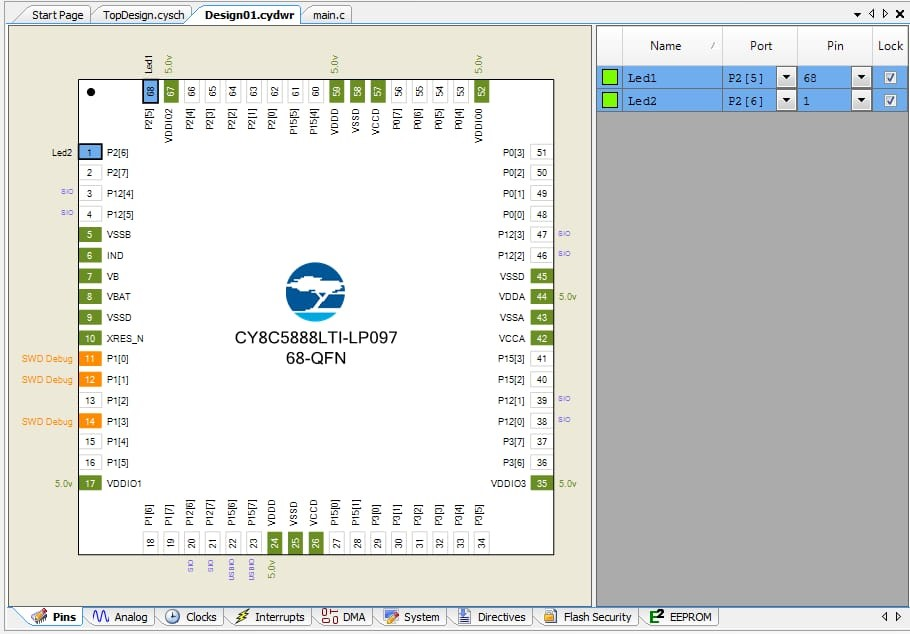
\includegraphics[width=5cm]{images/broche2.jpg }
         \caption{Affectation des broches }
         \label{fig:example7}
       \end{figure}
     \item \textbf{Ecrire le code du projet fichier main.c}
     Grace a l'IDE PSoC, nous avons utilisé une approche graphique pour configurer le compteur à sept segments.
  Nous avons utilisé des composants spécifiques pour contrôler les segments de l'afficheur et créer le compteur.

  \begin{figure}[htp]
    \centering
    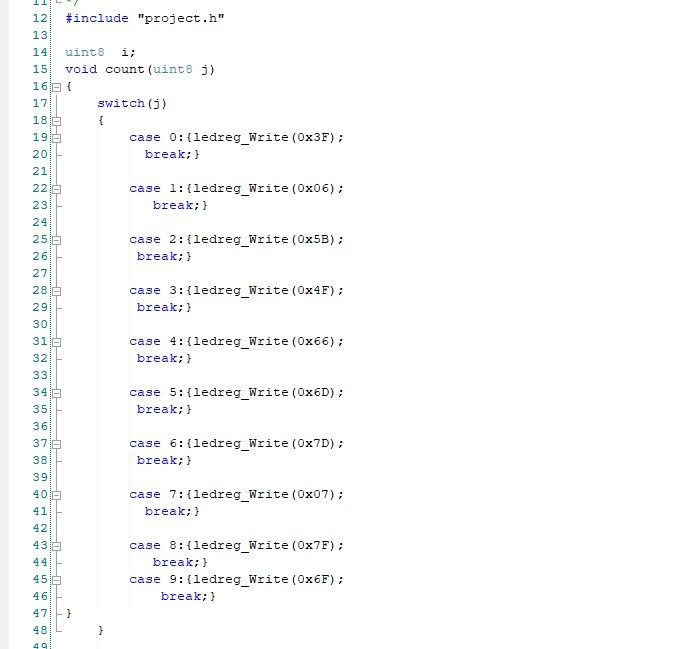
\includegraphics[width=10cm]{images/codetree.jpg }
    \caption{Address de tout les chiffres de 0 à 9 }
    \label{fig:example11}
  \end{figure}
\newpage
     \begin{figure}[htp]
         \centering
         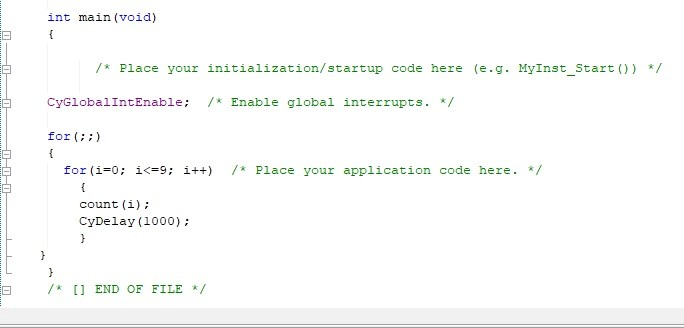
\includegraphics[width=10cm]{images/boucle.jpg }
         \caption{Boucle for pour le comptage }
         \label{fig:example12}
       \end{figure}
    
     \item \textbf{Effectuer le montage et Televersement }
     \begin{figure}[htp]
        \centering
        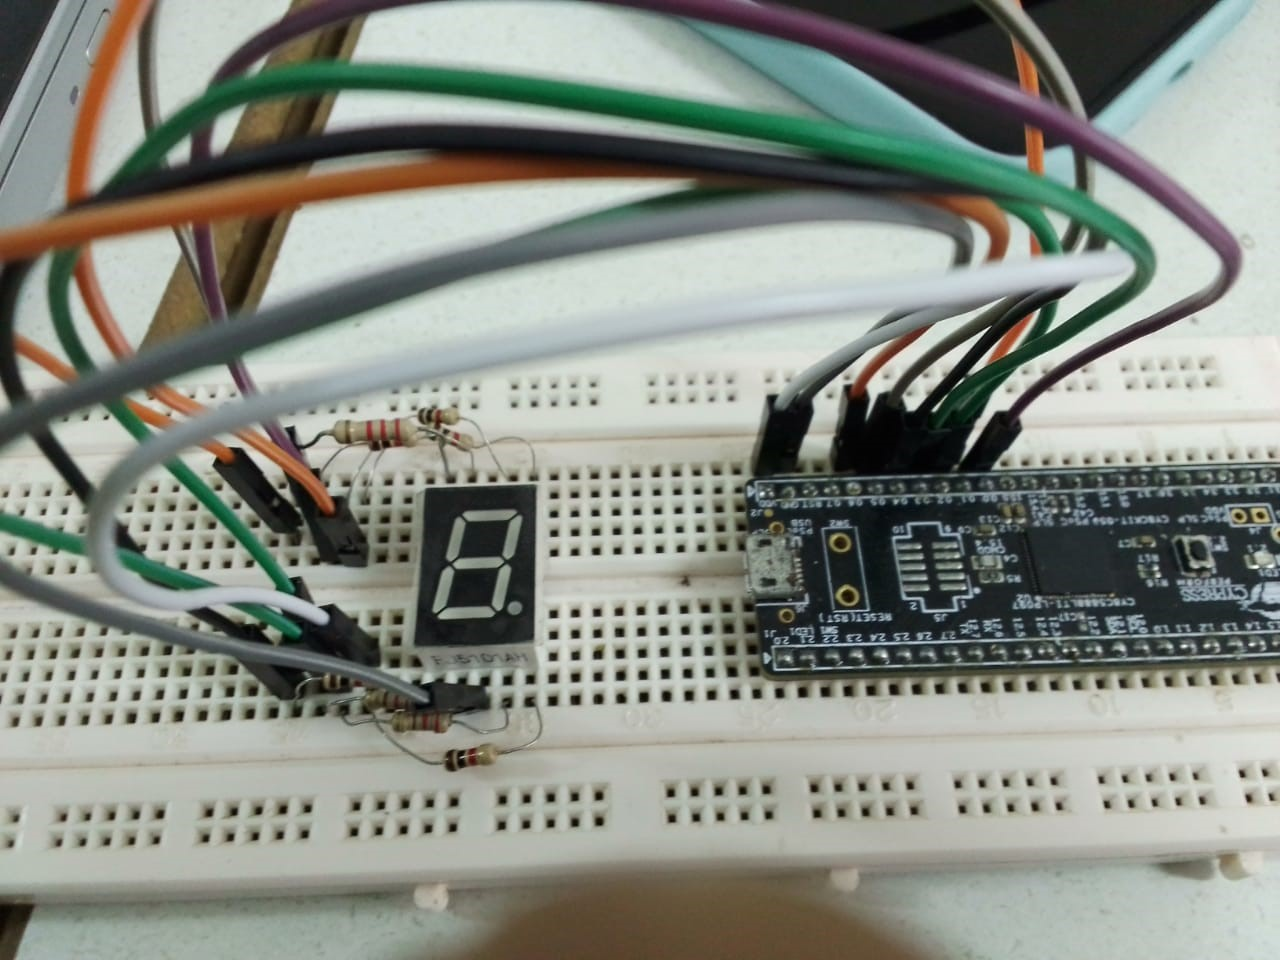
\includegraphics[width=10cm]{images/cablage.jpg }
        \caption{Schema cablage 7 seg à anodes commune }
        \label{fig:example13}
      \end{figure}
 \end{itemize}
 
 \subsection{Résultat obtenue}
 \label{sec:Résultat obtenue}
 Après avoir configuré et programmé le PSoC, nous avons observé que le
  compteur à sept segments fonctionnait comme prévu. Il s'incrémentait de
   manière croissante en affichant les chiffres de 0 à 9 sur l'afficheur
    à sept segments. Chaque chiffre était affiché 
 pendant une durée , puis le compteur passait au chiffre suivant. 
 \begin{figure}[htp]
     \centering
     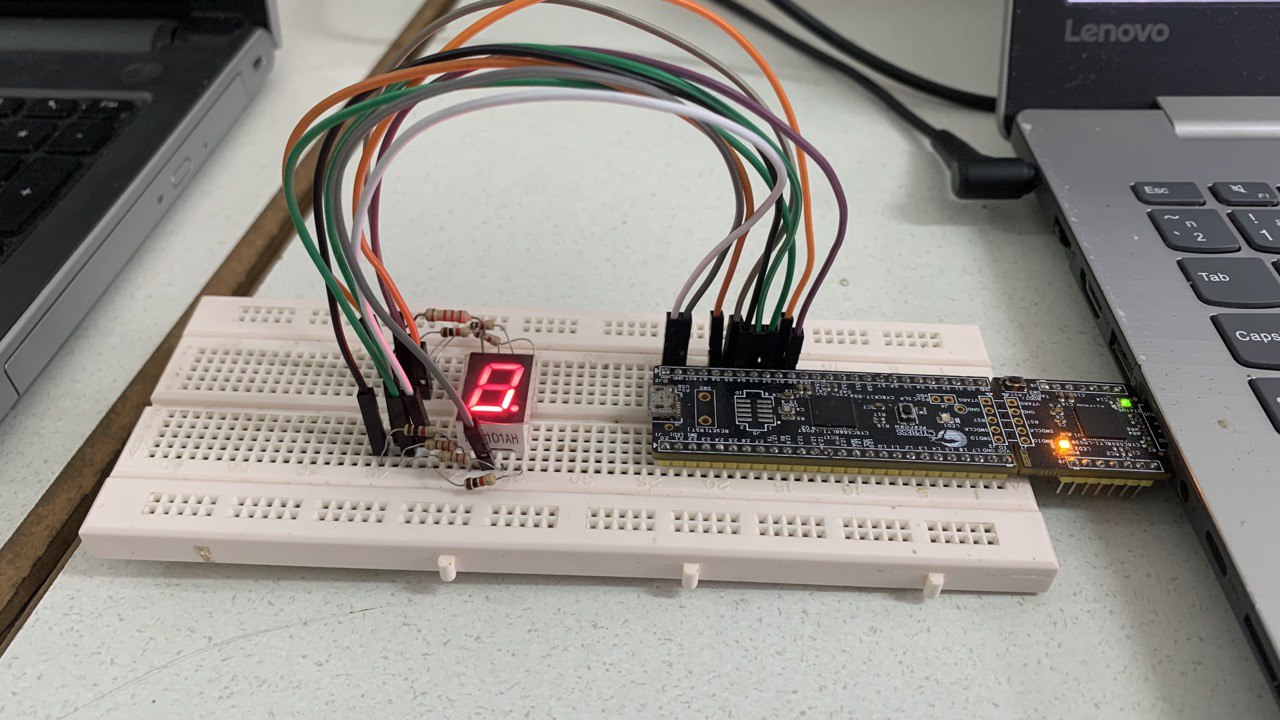
\includegraphics[width=10cm]{images/7seg.jpg }
     \caption{ Resultat:comptage}
     \label{fig:example14}
   \end{figure}
 
  \newpage
 \subsection{Interpretation}
 \label{sec:Interpretation}
 \todo[inline]{Le PSoC peut etre utilisé dans les compteurs, les horloges, les minuteries,
  les dispositifs de mesure et autres applications où un affichage numérique 
  est nécessaire.L'objectif principal de cette activité etait de compter et d'afficher 
  des chiffres de manière séquentielle sur l'afficheur à sept segments
 }
 \section{Activité n°4 :Message défilant sur un afficheur LCD }
 \label{chap:Activité n°3 :Message défilant sur un afficheur LCD }
 Dans ce projet, le PSoC sera utilisé pour générer les signaux de contrôle
  nécessaires pour l'afficheur LCD et transmettre les données à afficher. 
  Le PSoC offre une grande flexibilité et des fonctionnalités intégrées,
  ce qui facilite la gestion de l'interface avec l'afficheur LCD.
 \subsection{Etude Theorique}
 \label{sec:Etude Theorique}
 \begin{itemize}
     \item \textcolor{red}{\textbf{Configuration matérielle:}}
    Choisir un afficheur LCD compatible avec le PSoC, en tenant compte du nombre de caractères et de lignes
      nécessaires pour votre application
     \item \textcolor{red}{\textbf{Configuration logicielle:}}l'environnement de développement intégré (IDE) du PSoC
      comme PSoC Creator,choisir la bonne carte et créez un nouveau projet.
 \end{itemize}
 
 
 \subsection{Manipulation}
 \label{sec:Manipulation}
 \begin{itemize}
     \item \textbf{Lancer le logiciel Psoc Creator:}
     Lancez PSoC Designer et créez un nouveau projet en sélectionnant 
     le microcontrôleur PSoC adapté à votre modèle spécifique.
     \item \textbf{Ajoutez les composants nécessaires: } 
     Dans l'onglet "Component Catalog"
     recherchez et ajoutez les composants requis pour les deux diodes
     \begin{figure}[htp]
         \centering
         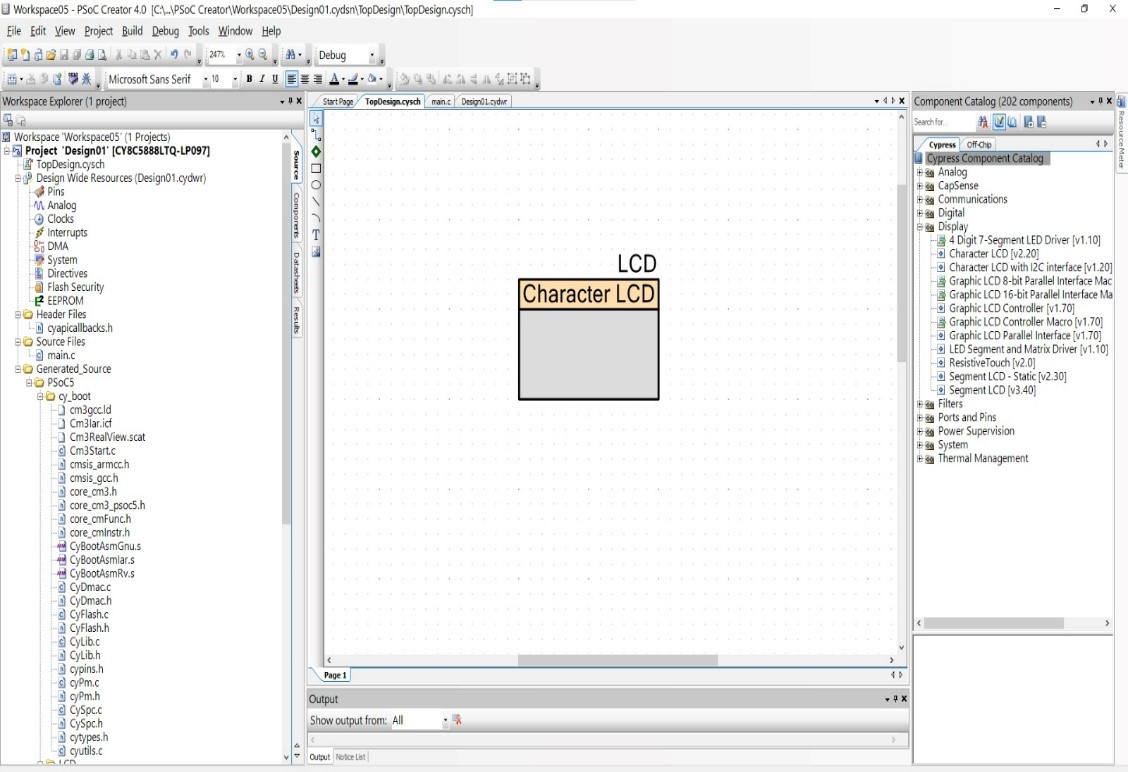
\includegraphics[width=10cm]{images/schema4.jpg }
         \caption{Schema pour LCD }
         \label{fig:example15}
       \end{figure}
       \newpage
     \item \textbf{Configuration des broches de sortie dans .cydwr}\\
     Veillé à ce que les broches soient définies en mode numérique et en tant que sorties.
    
     \begin{figure}[htp]
         \centering
         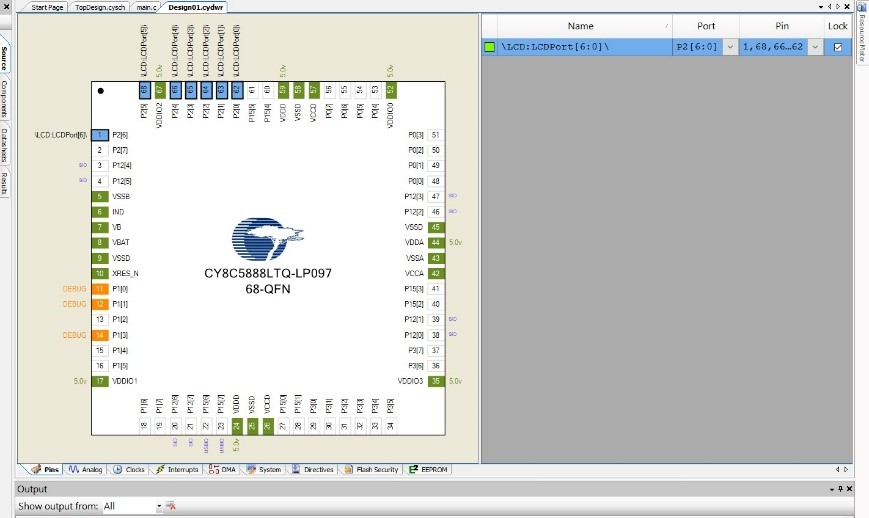
\includegraphics[width=10cm]{images/broche4.jpg }
         \caption{Affectation des broches }
         \label{fig:example16}
       \end{figure}
     \item \textbf{Ecrire le code du projet fichier main.c}\\
     Utilisant l'IDE PSoC, nous avons écrit du code pour créer le message défilant sur l'afficheur LCD.
     Nous avons utilisé des instructions spécifiques pour envoyer les caractères du message sur les lignes de données de l'afficheur LCD et contrôler les signaux de contrôle appropriés pour le défilement.
     
  \begin{figure}[htp]
    \centering
    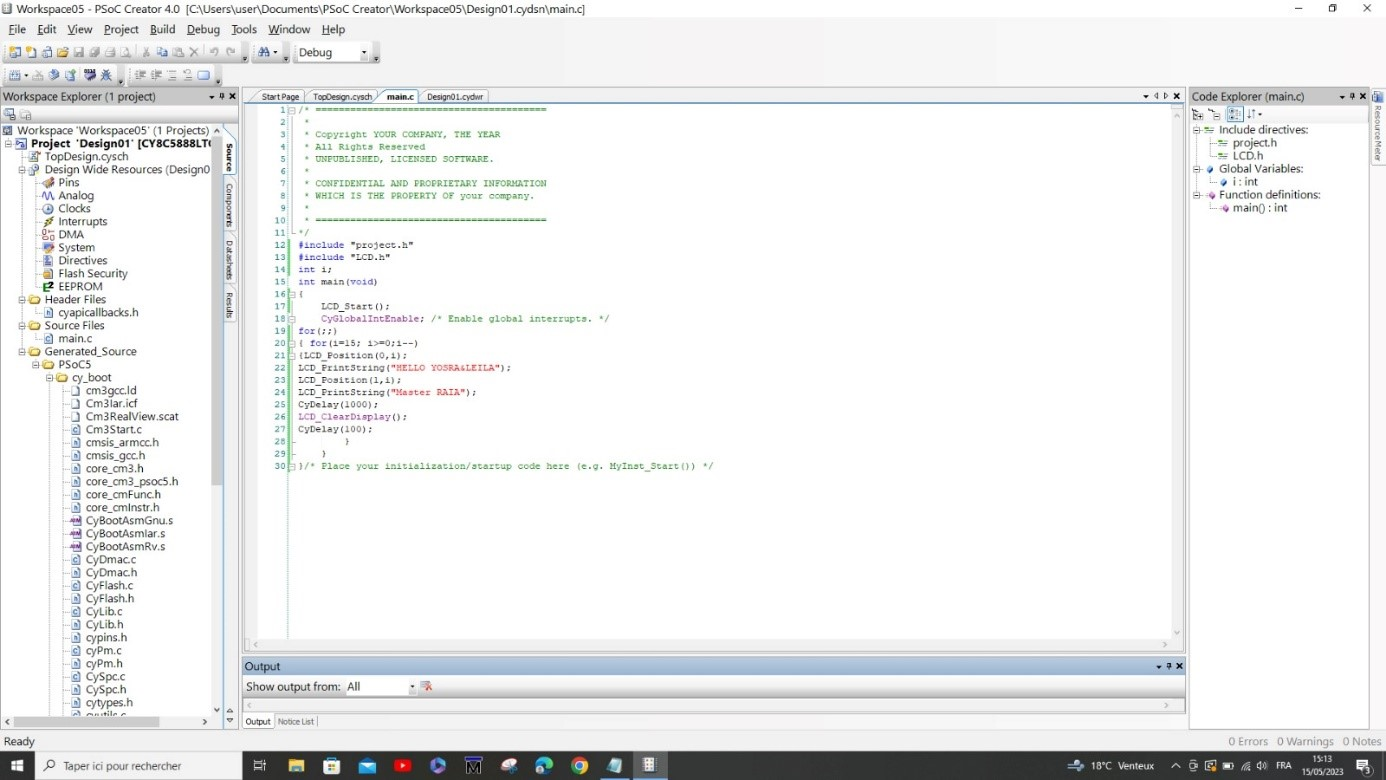
\includegraphics[width=10cm]{images/code4.jpg }
    \caption{Code pour LCD}
    \label{fig:example16}
  \end{figure}
  \newpage
     \item \textbf{Effectuer le montage et Televersement }
     \begin{figure}[htp]
        \centering
        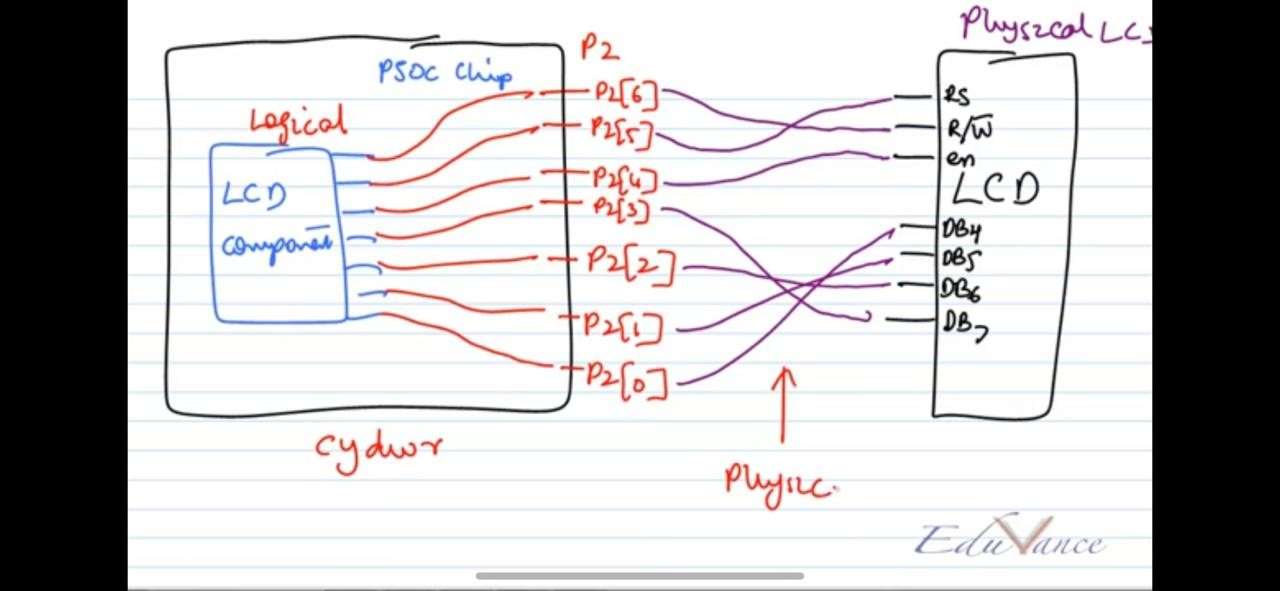
\includegraphics[width=10cm]{images/cablage4.jpg }
        \caption{Schema cablage LCD }
        \label{fig:example17}
      \end{figure}
 \end{itemize}
 \newpage
 \subsection{Résultat obtenue}
 \label{sec:Résultat obtenue}
 Après avoir configuré et programmé le PSoC, 
 nous avons observé que le message se défilait de manière fluide sur
  l'afficheur LCD. Le texte s'affichait progressivement sur l'écran,
   puis se déplaçait horizontalement pour laisser place aux caractères
    suivants. Ce processus se répétait pour créer l'effet de défilement 
    continu du message.
 \begin{figure}[htp]
     \centering
     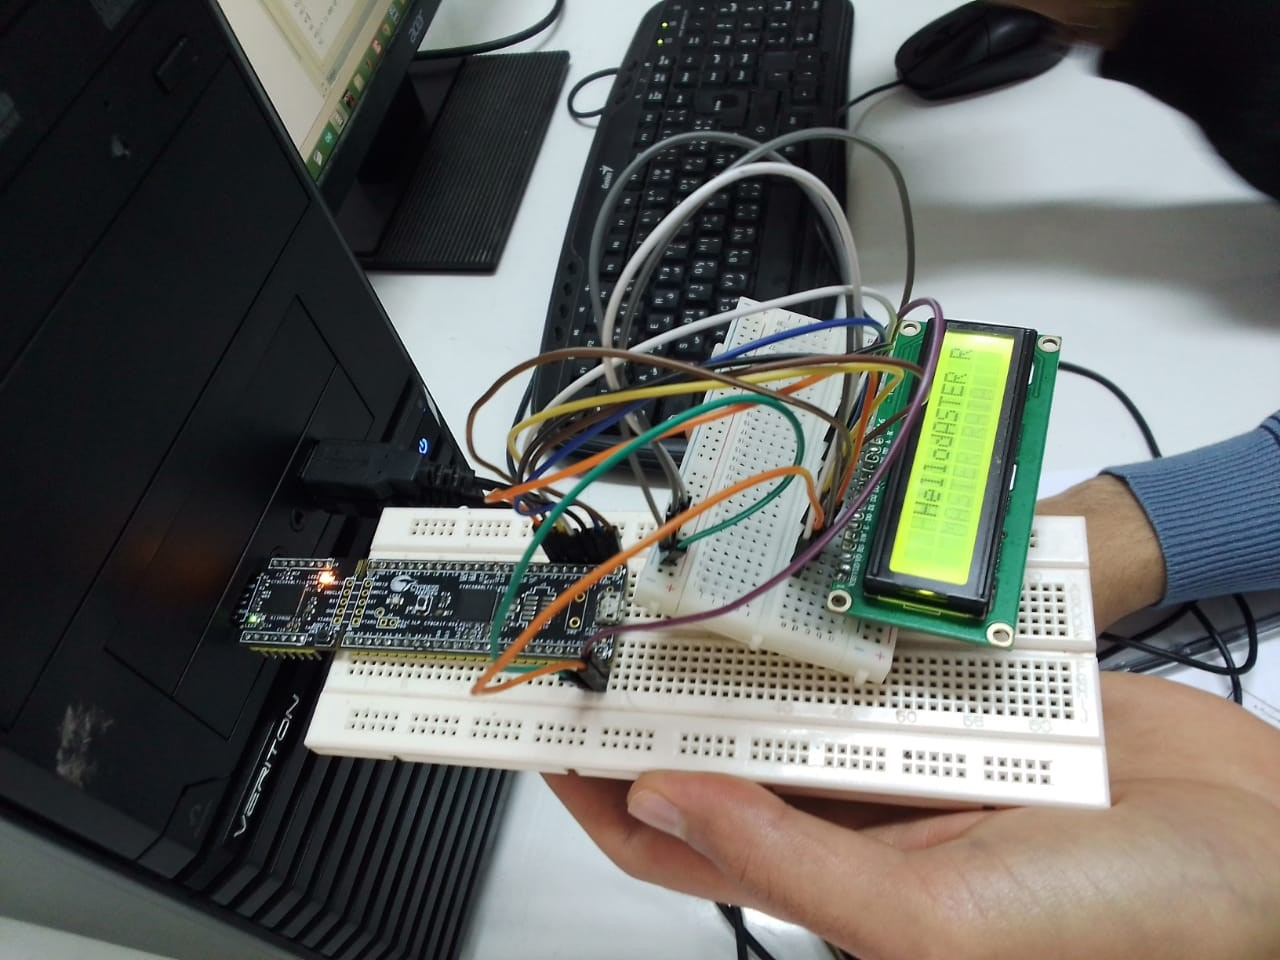
\includegraphics[width=10cm]{images/resultat4.jpg }
     \caption{ Resultat:Message Defillant}
     \label{fig:example18}
   \end{figure}
 
  
 \subsection{Interpretation}
 \label{sec:Interpretation}
 \todo[inline]{Cette Activité vise à créer un système qui utilise un PSoC pour contrôler un afficheur LCD
 et afficher des informations textuelles ou numériques. Les afficheurs LCD sont couramment utilisés dans divers appareils
  électroniques pour afficher des messages, des données ou des états.
L'objectif principal de ce projet est de contrôler et d'afficher du texte ou des chiffres sur l'afficheur LCD à l'aide du PSoC

 }


\section{Conclusion}
\label{chap:conclusion}

\textbf{En conclusion, les activités realisées, tels que le clignotement de LED
 en alternance, le compteur à sept segments et l'afficheur LCD avec un PSoC, 
 démontrent la polyvalence et les capacités du PSoC en tant que système sur puce
  programmable. Ces projets nous offres des opportunités d'apprentissage pratiques pour
et ne constitue qu'une initiation au monde des circuits programmables FPGA.Nous devons donc explorer encore plus les fonctionnalités du PSoC et 
   créer des applications interactives.}
